% Capítulo 6
\chapter{Estudo Experimental}
\label{cap:cap6}

Este capítulo consiste em apresentar o estudo experimental realizado, envolve a concepção do contexto de experimentação, das configurações e características dos elementos envolvidos, a seleção das variáveis influenciadoras, o controle e instrumentalização do experimento, sua execução e captura de dados durante experimentação, e por fim, a análise e conclusões obtidas a partir desses resultados. 

O objetivo do experimento é analisar por meio de demonstração da taxonomia proposta, a viabilidade do uso de mecanismos de \textit{throttling} como candidato para aumentar a disponibilidade dos elementos presentes em \textit{IoT} através do ajuste de comportamento por ação de limiares de atuação que consideram seus aspectos energéticos para assim,  prolongar a autonomia energética dos dispositivos. A abordagem é aderente e cobre os elementos presentes na taxonomia proposta no Capítulo \ref{cap:cap4} permitindo comparação e análise entre dispositivos que diferem sobre o fato de terem sua operação ajustada mediante \textit{throttling} ou não. 

\section{Metodologia}

O experimento compara os efeitos do mecanismo de \textit{throttling} em dispositivos com capacidade de coleta de energia, com foco em examinar a disponibilidade de cada um voltado aos aspectos energéticos em condições de atuação semelhante.

\begin{figure}[H]
	\centering
	\caption{Processo de Estudo Experimental.}
	\label{fig:cap6metodologia}
	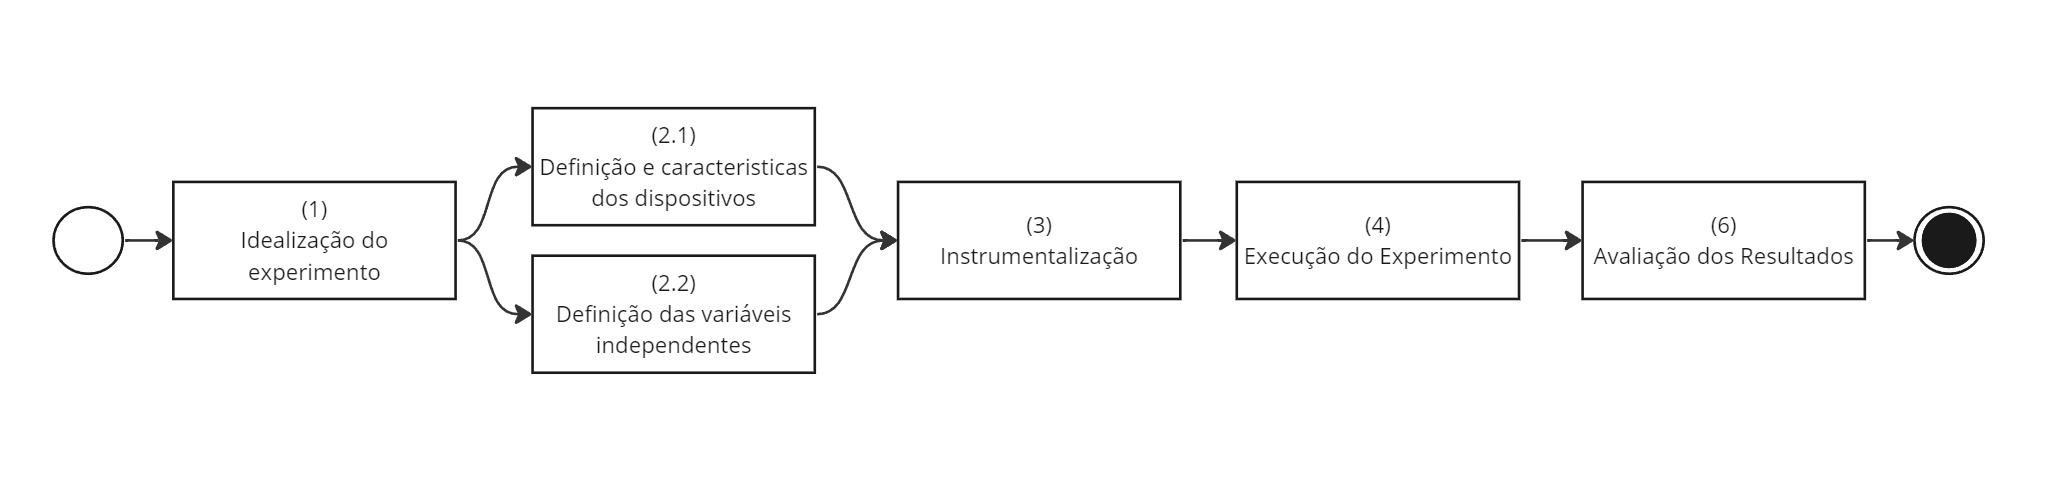
\includegraphics[width=1\linewidth]{Imagens/cap6/cap6metodologia.jpg}
	
	Fonte: elaborado pelo autor.
\end{figure} 

Para tal, buscou-se observar a influência do fator limitante na alteração de comportamento dos participantes em resposta aos valores obtidos como energia coletada e por sua vez, reserva energética. Além disso, almeja-se compreender sua eficiência na tomada de decisão em atender ou não às solicitações, em virtude da autoanálise de suas capacidades à medida que há variação de oferta energética disponível. Este estudo visa analisar o uso de \textit{throttling} como solução para estender a disponibilidade em relação aos fatores energéticos dos dispositivos com capacidade de coleta energética. 

A Figura \ref{fig:cap6metodologia} apresenta os processos executados e sua ordem exprime a precedência para realização das etapas adjacentes. Na Seção \ref{cap6:idealizacao}, foi concebido a idealização do experimento (Etapa 1), quais os requisitos do projeto para viabilizar a análise e comparação de dispositivos com padrão \textit{throttling}. Partindo daí, foi projetado um ambiente para abstrair os elementos envolvidos, buscando garantir o controle na equidade de condições para os dispositivos observados. Todo o processo foi viabilizado pelo uso da plataforma Docker\footnote{Disponível em \url{https://www.docker.com/}.}, uma plataforma de virtualização que atua sobre o desenvolvimento, envio e execução de aplicativos organizados na forma de contêineres e por esses fatores, atende às restrições necessárias de encapsulamento para cada aplicação e suas dependências auto contidas. 

A abordagem utilizando \textit{containers} permitiu que os dispositivos fossem estimulados simultaneamente, mantendo controle sobre seus recursos garantindo os termos da operação. Sendo assim, a definição dos dispositivos e variáveis (Etapa 2) do experimento considera:  I - Dispositivos simulados com capacidade de coleta e armazenamento de energia estão inseridos em um dado ambiente similar ao uso real; II - Os dispositivos recebem, ao mesmo tempo, um valor como coleta de energia; III - Os dispositivos participantes possuem a mesma capacidade para armazenar energia coletada em \textit{storage}; IV - Os dispositivos são submetidos ao mesmo tipo de solicitações simultaneamente.

Na Instrumentalização (Etapa 3), capacita o experimento para coletar, apresentar e preservar os resultados aferidos de uma execução e posterior visualização dos dados obtidos, os detalhes estão descritos na Seção \ref{cap6:instrumentalizacao}. A Seção \ref{cap6:execucao} descreve apropriadamente os detalhes de execução (Etapa 4). Neste ponto, todas as etapas planejadas anteriormente no andamento do processo ja foram abordados. Em decorrência disso, habilita-se o experimento para realizar múltiplas execuções conforme protocolo estabelecido, aplicando os estímulos já definidos (carga de solicitações e disponibilização de recursos energéticos),  coletando os resultados obtidos.

Em seguida, a Seção \ref{cap6:avaliacao}, apresenta a avaliação dos resultados (Etapa 5), que consiste na descrição e análise dos dados obtidos durante a execução. Os dados analisados são compostos pelos valores inferidos ao grupo de variáveis independentes e os resultados obtidos no grupo de variáveis dependentes. Constituem as variáveis independentes: os valores energéticos disponibilizados; e da quantidade de solicitações realizadas. A análise se fundamenta em observar como o mecanismo \textit{throttling} implementado no dispositivo se colocará como agente atenuante do gasto energético utilizado a medida seus limiares de atuação são atingidos de acordo com o modo de operação previsto para determinados fatores observáveis presentes.

Finalmente, encerrando a execução do experimento, as variáveis dependentes resultantes são coletadas para avaliação e evidenciam: a performance em relação a quantidade total de solicitações atendidas ao fim da execução do experimento e a quantidade de solicitações impedidas mediante indisponibilidade de recursos em \textit{storage}. Ao aprofundar a análise, é preciso ainda, contrapor os dados temporais de oferta energética em relação a quantidade presente no dispositivo, o que justificará a atuação de limitadores e sua capacidade em manter um dispositivo operacional do ponto de vista energético.


\section{Idealização}
\label{cap6:idealizacao}
Uma vez definido os objetivos do experimento, a idealização é o ponto onde foi construído as bases de execução do estudo. Assim, foram concebidas a estruturação geral dos parâmetros, a  definição do cenário para realizar os testes, além da capacidade de coleta dos resultados e avaliação de conformidade com os termos presentes na taxonomia proposta.

O cenário foi idealizado para simular a atuação de dispositivos em dado ambiente. Aqui, fundamentalmente, dispositivos provedores devem atender as solicitações de operações à medida que são providos energeticamente por seu sistema de coleta (\textit{power supply}). Decorrente disso, cabe ao dispositivo, com base nas condições energéticas presentes em seu armazenamento (\textit{storage}), decidir se é capaz ou não de realizar a operação solicitada. Para atingir seu objetivo, o mecanismo de \textit{throttling} deverá atuar conforme instancia de observação referente às classes taxonômicas ja vistas na Figura \ref{fig:cap4divisaobasetaxonomia}.

Para sua concepção é preciso definir alguns pontos primários esperados. Assim descreve-se \( C_a \) como o valor consumido pelo dispositivo quando estado ativo, \( C_i \), o consumo enquanto estado inativo e \( C_h \) representa dispositivos sem capacidade energética, com seu valor é zero e configura um equipamento em estado hibernativo. 

Seja o tempo a duração de um ciclo $T(c)$, obtido pela soma da duração do tempo onde o dispositivo esta ativo \( t_a \), permanece inativo \( t_i \) além do tempo que hiberna \( t_h \), é seguro expressar o tempo total do ciclo em razão dos constituintes na expressão $T(c_n) = $ \( t_a + t_i + t_h \). O consumo total $C_{total}$, durante um ciclo é obtido de maneira que:
\[C_{total} = C_a \cdot t_a + C_i \cdot t_i + C_h \cdot t_h \quad (\text{Sendo }C_h = 0)\]
\[C_{total} = C_a \cdot t_a + C_i \cdot t_i\]
Assim, considerando um dispositivo que permaneça ativo durante todo o ciclo \( t_a = T \), \( t_i = 0 \), \( t_h = 0 \):
\[ C_{total} = C_a \cdot T \]
De outra forma, caso permaneça hibernando durante todo o ciclo \( t_h = T \), teremos seu consumo total:
\[ C_{total} = C_t \cdot T = 0 \]

Portanto, um dispositivo com ação do mecanismo \textit{throttling} deverá ter seu comportamento adequado ao modo de atuação esperado, através da recusa de solicitações em ciclos proporcionando a variação entre $ t_a, t_i \ e\ t_h$ cooperando com o motivo de atuação para que reduza seu consumo, assim conduzindo o dispositivo ao cenário onde o tempo de atividade é cada vez menor ao tempo total do ciclo \( t_a < T \) e, se necessário, manter $t_h \approx 0$.

Ainda nesta etapa, foi necessário conceber uma configuração de componentes adequadas que pudessem representar um dispositivo com capacidade de coleta energética. Com esse objetivo, reduziu-se o dispositivo aos aspectos de armazenamento (\textit{storage}), sua entrada energética simulando um valor coletado através de um \textit{power supply} e os demais componentes necessários para uma operação. Assim, a dinâmica energética segue-se ao passo que um valor energético é apresentado em ciclos ao \textit{storage}, que armazena e fornece os valores para uso dos demais componentes presentes. A Figura \ref{fig:cap6dinamica} ilustra dinâmica energética de funcionamento do dispositivo.

\begin{figure}[H]
	\centering
	
	\caption{Dinâmica do fornecimento energético Dispositivo Provedor.}
	\label{fig:cap6dinamica}
	\noindent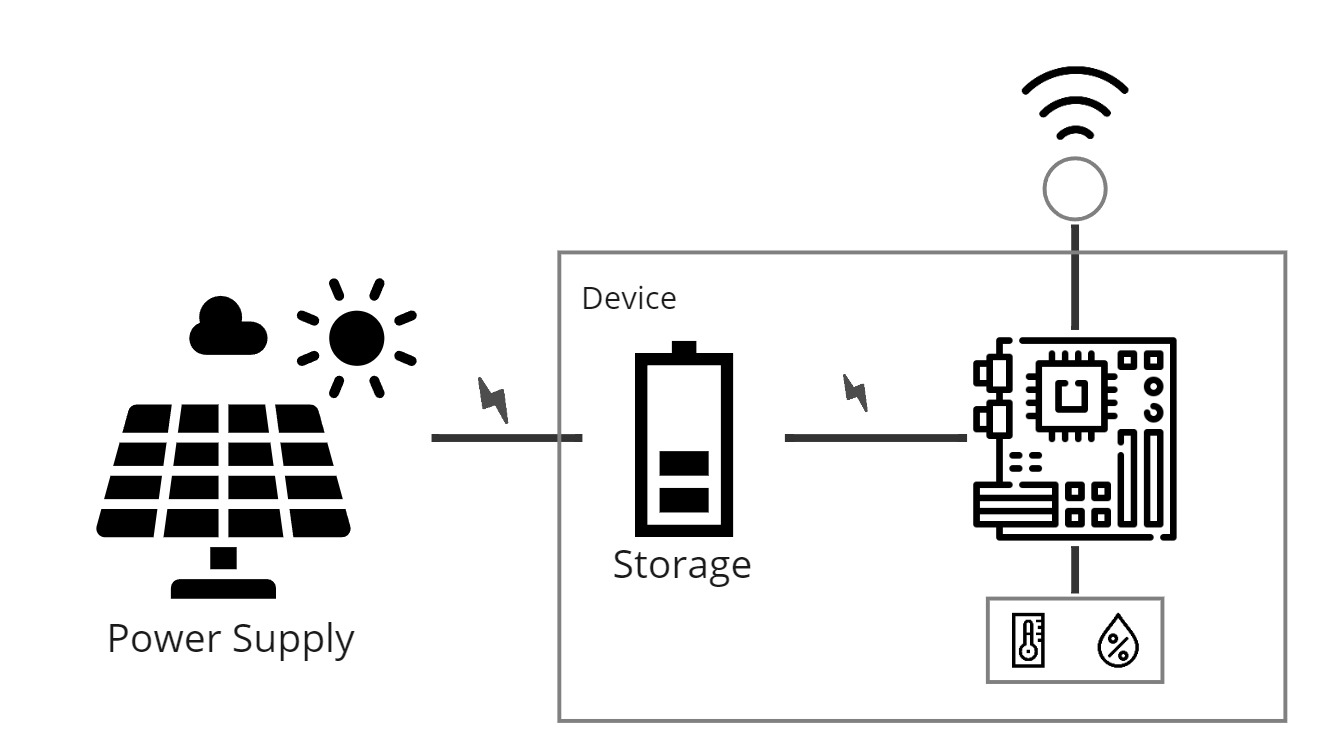
\includegraphics[width=0.75\linewidth]{Imagens/cap6/cap6dinamica.jpg} 
		
	Fonte: elaborado pelo autor.
\end{figure}


Em consequência, acontecendo disponibilidade energética, cabe ao dispositivo armazena-la na medida que os valores vão sendo apresentados, respeitando sua capacidade de armazenamento. Ao passo que paralelamente, os valores energéticos estão disponibilizados na forma de recurso ofertado e utilizado na medida que realiza suas operações.

Finalmente, o dispositivo deverá em todo seu funcionamento atuar dinamicamente em conformidade com os modo de operação projetados que representem os valores de recursos energéticos que possui. No experimento estão cobertos quatro modos de atuação a depender das capacidades energéticas:

\begin{enumerate}	
\item Modo Abundante:  representa o dispositivo que possui recursos energéticos amplamente disponíveis, permitindo o funcionamento completo e otimizado de todas as suas funcionalidades. Aqui, atenderá quaisquer solicitação enviada, sem atuação do mecanismo limitante, aproveitando ao máximo a disponibilidade de energia;
\item Modo Atenção: Uma vez atingido este patamar, o dispositivo ainda apresenta condição energética razoável, porém moderadamente restringirá algumas operações atendidas com a motivação de preservar parte dos recursos até que um novo cenário energético seja apresentado;
\item Modo Alerta: alcançado quando o dispositivo está operando com recursos energéticos extremamente limitados. Algumas operações ainda podem ser realizadas (conforme privilégios das operações ou solicitantes). Este modo motiva-se na intenção de prolongar a funcionalidade básica do dispositivo a todo custo enquanto tenta evitar a entrada no Modo Hibernação. 
\item Modo Hibernação: este modo é ativado quando não possui mais recursos energéticos disponíveis para realizar operações. O dispositivo entrará em um estado de hibernação ou equivalente até que recursos energéticos sejam recuperados. Nenhuma ação de limitação acontecerá durante esse modo, caso hiberne,  o dispositivo encontra-se esgotado energeticamente.
\end{enumerate}

Um modo de operação guiará como o mecanismo de \textit{throttling} atua em detrimento do valor disposto em sua reserva energética, assim pode contribuir reduzindo a utilização dos recursos, amortizando ou interrompendo o uso energético nos serviços ofertados no dispositivo a medida que limita à capacidade de atendimento as solicitações. 

Naturalmente, os modos de operação podem sofrer variação, cabe a análise das especificidades e natureza que se destina cada implementação, para assim, dado o exame desses fatores, definir apropriadamente quais modos serão necessários para o dispositivo almejado. Estes modos guiam a capacidade de mudança dos estados do dispositivo. Uma vez que, são justificados por tal modo  reduzir a quantidade de solicitações atendidas, proporcionando momento em estado de inatividade forçada contribuindo para redução dos recursos utilizados. De maneira geral, a dinâmica dos estados do dispositivo pode ser visualizada na Figura \ref{fig:cap6maquinaestados}. 

\begin{figure}[H]
	\centering
	
	\caption{Máquina de estados do Dispositivo.}
	\label{fig:cap6maquinaestados}
	\noindent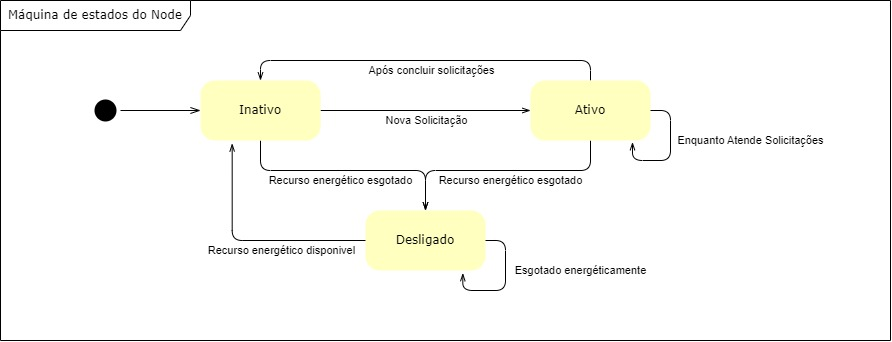
\includegraphics[width=0.75\linewidth]{Imagens/cap6/cap6maquinaestados.jpg} 
	
	Fonte: elaborado pelo autor.
\end{figure}

A relação entre modos de operação e estados deixa implícita presença do mecanismo limitante e atuação implementada em cada modo, contribuindo para que o dispositivo permaneça em um estado de inatividade à depender das condições estabelecidas em que se encontra com a motivação de preservar ou restabelecer sua condição energética. Sendo assim, uma vez em determinado modo, o dispositivo terá uma quantidade potencial para atendimento das operações e estas, colocam o dispositivo em um estado ativo. Caso atinja valor limitador de acordo com o modo, novas operações passam a ser negadas e por sua vez, colocará dispositivo em inatividade, reduzindo assim seu gasto energético.

Para fins de experimentação, os estados possíveis para o dispositivo são descritos como:
\begin{itemize}
	\item Estado Inativo: Aqui o dispositivo estará consumindo a menor quantidade de recurso energético possível. Enquanto inativo, encontra-se ocioso sem realizar nenhuma tarefa à medida que aguarda novas solicitações ou seja o caso necessário, aguarde nova entrada energética disponível, para atender solicitações anteriormente recusadas.
	\item Estado Ativo: Um dispositivo é considerado ativo enquanto atende solicitações. Nesse estado o dispositivo utilizará os recursos energéticos necessários para realização das atividades mediante o consumo desses recursos. 
	
	\item Estado Hibernando: No experimento, o estado hibernando é a indicação que o dispositivo não tem mais capacidade de assumir qualquer outro estado enquanto não receber recursos energéticos, seja por modo contundente de preservação ou em decorrência do esgotamento de suas reservas. Portanto, neste estado, um dispositivo não realizará qualquer atividade.	
	
\end{itemize}




\section{Definição das Variáveis Independentes}
\label{cap6:variaveisdispositivos}
Dispositivos com a capacidade de coleta de energia (\acl{EHS}) se baseiam na utilização de fontes energéticas disponíveis no ambiente para suprir, parcial ou totalmente, a demanda de um dispositivo. Em todo caso, para o experimento, não há, a princípio, a intenção de analisar as particularidades de alguma fonte energética, sua natureza e características de uso ou eficiência. 

Todavia, na execução do experimento é necessário a compreensão sobre à disponibilidade da oferta energética em termos quantitativos de uma fonte qualquer. Para cobrir os critérios levantados na taxonomia como capacidade de coleta, os dados utilizados se assemelham ao comportamento observado por um fonte de energia solar e foram concebidos à partir de adaptação dos dados reais disponibilizados no Atlas Brasileiro de Energia Solar \cite{martins2017atlas}. Em destaque, a definição dos valores foi orientada pela referencia para cidade de Natal/RN como média diária de irradiação solar no decorrer dos meses. Adaptado ao experimento, cada valor apresentado compreenderá à uma jornada $J_i$ (para $i = 1,2,...,12$), totalizando 12 jornadas. Para viabilizar o experimento, os valores originários foram tratados como parâmetro de quantidade, desprezando sua grandeza. Assim,  Conforme Tabela \ref{table:cap6distribuicaonatal} onde cada valor representa o montante energético disponibilizado em uma respectiva jornada distribuídos em ciclos.

\begingroup

\setlength{\tabcolsep}{10pt} % Default value: 6pt
\renewcommand{\arraystretch}{1.5} % Default value: 1

\begin{table}[h]
	
	\centering
	\caption{Valores ofertados por ciclo}
	\smaller[8]
	\tabcolsep=0.1cm
\begin{tabular}{ r | *{13}{c} }
	\toprule
        &  \multicolumn{13}{c}{Disponibilizado no Ciclo (c)}\\\cline{2-14}
	Jornada (J) & \begin{tabular}{@{}c@{}} c05 \\(0.007)\end{tabular} &
	\begin{tabular}{@{}c@{}} c06 \\(0.02) \end{tabular}	& 
	\begin{tabular}{@{}c@{}} c07 \\(0.053)\end{tabular} &
	\begin{tabular}{@{}c@{}} c08 \\(0.087) \end{tabular}&
	\begin{tabular}{@{}c@{}} c09 \\(0.105) \end{tabular}&
	\begin{tabular}{@{}c@{}} c10 \\(0.127) \end{tabular}& 
	\begin{tabular}{@{}c@{}} c11 \\(0.136) \end{tabular}& 
	\begin{tabular}{@{}c@{}} c12 \\(0.125) \end{tabular}& 
	\begin{tabular}{@{}c@{}} c13 \\(0.12) \end{tabular}& 
	\begin{tabular}{@{}c@{}} c14 \\(0.101) \end{tabular}& 
	\begin{tabular}{@{}c@{}} c15 \\(0.074)\end{tabular}& 
	\begin{tabular}{@{}c@{}} c16 \\(0.04)\end{tabular}&
	\begin{tabular}{@{}c@{}} c17 \\(0.005)\end{tabular}\\
	
	\hline
	J01 5674 & 39.72 & 113.48 & 300.72 & 493.64 & 595.77 & 720.6 & 771.66 & 709.25 & 680.88 & 573.07 & 419.88 & 226.96 & 28.37\\
	\hline
	J02 6017 & 42.12 & 120.34 & 318.9 & 523.48 & 631.78 & 764.16 & 818.31 & 752.12 & 722.04 & 607.72 & 445.26 & 240.68 & 30.09 \\
	\hline
	J03 6032 &  42.22 & 120.64 & 319.7 & 524.78 & 633.36 & 766.06 & 820.35 & 754.0 & 723.84 & 609.23 & 446.37 & 241.28 & 30.16 \\
	\hline
	J04 6082 & 42.57 & 121.64 & 322.35 & 529.13 & 638.61 & 772.41 & 827.15 & 760.25 & 729.84 & 614.28 & 450.07 & 243.28 & 30.41 \\
	\hline
	J05 5561 & 38.93 & 111.22 & 294.73 & 483.81 & 583.9 & 706.25 & 756.3 & 695.12 & 667.32 & 561.66 & 411.51 & 222.44 & 27.8\\
	\hline
	J06 5075 & 35.52 & 101.5 & 268.97 & 441.52 & 532.88 & 644.52 & 690.2 & 634.38 & 609.0 & 512.58 & 375.55 & 203.0 & 25.38 \\
	\hline
	J07 4658 & 32.61 & 93.16 & 246.87 & 405.25 & 489.09 & 591.57 & 633.49 & 582.25 & 558.96 & 470.46 & 344.69 & 186.32 & 23.29 \\
	\hline
	J08 4773 & 33.41 & 95.46 & 252.97 & 415.25 & 501.16 & 606.17 & 649.13 & 596.62 & 572.76 & 482.07 & 353.2 & 190.92 & 23.87\\
	\hline
	J09 5571 & 39.0 & 111.42 & 295.26 & 484.68 & 584.95 & 707.52 & 757.66 & 696.38 & 668.52 & 562.67 & 412.25 & 222.84 & 27.86\\
	\hline
	J10 5971 & 41.8 & 119.42 & 316.46 & 519.48 & 626.95 & 758.32 & 812.06 & 746.38 & 716.52 & 603.07 & 441.85 & 238.84 & 29.86 \\
	\hline
	J11 6112 & 42.78 & 122.24 & 323.94 & 531.74 & 641.76 & 776.22 & 831.23 & 764.0 & 733.44 & 617.31 & 452.29 & 244.48 & 30.56 \\
	\hline
	J12 6269 & 43.88 & 125.38 & 332.26 & 545.4 & 658.25 & 796.16 & 852.58 & 783.62 & 752.28 & 633.17 & 463.91 & 250.76 & 31.35 \\
\bottomrule
\end{tabular}
\label{table:cap6distribuicaonatal}
\\
\footnotesize Fonte: adaptado de \citeauthor{martins2017atlas}, (\citeyear{martins2017atlas})

\end{table}
\endgroup

O fator de distribuição atribuído a cada ciclo $c_i$ (para $i=0,1,2,...,23$) representa a medida que a oferta em dado instante $i$ tem em relação ao total esperado na jornada $J$ (na totalidade dos 24 ciclos), na qual pertence o ciclo. Para atribuição dos pesos dispostos, foi utilizado a referencia do material \citeonline{tutiempo2023} como equivalente de distribuição solar para um dia. Aqui, a limitação de adotar a distribuição solar especifica é justificada pela intenção de conceber os valores capazes de cobrir o objetivo do experimento, mesmo que aparentemente acaba por aproximar-se de termos que caracterizam propriamente os aspectos de oferta energética de fonte solar. 

Sendo assim, obteve-se a valoração das quantidades ofertadas, em referencia as jornadas e aplicados aos fatores de incidência encontrados para cada ciclo. Finalmente, é importante destacar ainda que os ciclos $c_0, c_1,... c_4$ e $c_{18}, c_{19},... c_{23}$ possuem peso atribuído nulo, porque representam ciclos onde não foi possível ofertar energia coletável significante, similar às características diurnas ou noturnas de fonte solar. para visualização Tabela \ref{table:cap6distribuicaonatal}, onde os valores desses ciclos em questão foram suprimidos.

O processo realizado para ofertar os valores ao \textit{storage} realiza-se uma vez definido o montante esperado para uma jornada e segue a partir disso, com o inicio do primeiro ciclo $c_{00}$ estendendo-se sequencialmente até fim do ciclo$c_{23}$, quando finda-se a jornada propriamente dita. Por sua vez, o próximo montante representará o principio do ciclo $c_{00}$ da jornada seguinte, realizando a mesma dinâmica de passagem de ciclos. Uma execução terminará quando todos os ciclos presentes nas jornadas sejam ofertadas e esta abordagem garante que todos os cenários previstos para o experimento são cobertos em sua execução e possibilita a geração e analise dos resultados obtidos.


Com a definição de comportamento dos ciclos e jornadas, determina-se também os processos realizados que cobrem uma dinâmica de oferta energética. Através disso, é possível abstrair qualquer tipo de fonte originária desde que seja possivel estimar e representar seu comportamento ao longo do tempo.

Partindo disso, surge a necessidade de caracterizar o processo de utilização desses recursos já armazenados. Uma segunda variável independente é necessária, o objetivo é realizar solicitações ao dispositivo de modo a estimular demanda para uso dos recursos. Assim, é preciso adotar algumas práticas para garantir que todos os dispositivos, além de receber a oferta energética estipulada como projetado, também sejam capazes de receber a mesma carga de solicitações que geram essas demandas, aproximadamente ao mesmo tempo. 

Na ação de atendimento de uma solicitação, o dispositivo é conduzido para iniciar ou permanecer em estado ativo, este estado intensifica a utilização de recursos quando comparado com estado inativo ou enquanto hiberna, já mencionado na Seção \ref{cap6:idealizacao}. Para cobrir essa dinâmica, após os dispositivos receberem a primeira oferta energética, no inicio da execução do experimento, inicia-se simultaneamente o processo continuo de envio das solicitações para cada dispositivo. Na razão aproximada de 1 solicitação a cada 0.2 segundos. Caso dispositivo não consiga receber uma solicitação, na janela de tempo, será considerado indisponível para aquele estimulo. 

Considera-se ainda que os termos necessários para transmissão ou as características da interface de comunicação podem exercer influência na razão de transmissão das solicitações, por este motivo é previsto que a quantidade total de solicitações realizadas pode sofrer pequena variação em relação ao esperado ao fim de cada execução do experimento. Em todo caso, é garantido em que todos os dispositivos foram estimulados ao mesmo total de solicitações durante a execução.

Finalmente, esta variável independente numérica, as solicitações realizadas, carrega o totais de requisições e em decorrência dela, observa-se os resultados obtidos para  quantidade total de solicitações realizadas que foram atendidas ou que encontraram o dispositivo indisponível.


\section{Definição dos Dispositivos}

Foi construído um modelo com a necessidade de representar um dispositivo \acs{IoT} embarcado com os mecanismos de \textit{throttling} necessários, este será uma implementação que deve receber ofertas energéticas em um cenário simulado, a medida que utiliza esses recursos para atender os estímulos das solicitações continuas providas em uma interface de acesso. A visão geral do dispositivo provedor e componentes pode ser visto na Figura \ref{fig:cap6providernode}. Além disso, o código fonte gerado para o mesmo está disponível no repositório Git\footnote{Código-Fonte do dispositivo provedor em \url{https://github.com/eusoupaulolopes/mst_experiments}.} aberto para análise e colaboração.

\begin{figure}[H]
	\centering
	
	\caption{Componentes do dispositivo Provedor.}
	\label{fig:cap6providernode}
	\noindent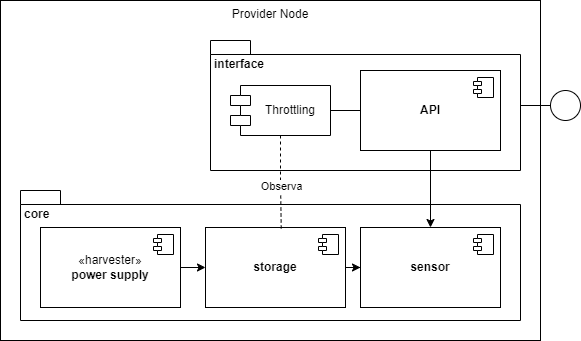
\includegraphics[width=0.75\linewidth]{Imagens/cap6/cap6providernode.png} 
	
	Fonte: elaborado pelo autor.
\end{figure}

Os elementos idealizados que constituem o dispositivo provedor são referentes aos seguintes componentes:
\begin{itemize}
	\item \textit{Power Supply} é caracterizado pela ação de fornecer os valores necessários para o funcionamento do dispositivo, simulando a coleta de energia no decorrer dos ciclos como descrito na Tabela \ref{table:cap6distribuicaonatal}. O componente atuará em paralelo a outras atividades realizadas pelo dispositivo. Caso o armazenamento do dispositivo esteja completamente cheio, ainda assim os valores de entrada serão entregues, caracterizando perdas. Por sua vez, o esgotamento energético do dispositivo não representa a incapacidade de receber novas entradas ofertadas e com isso, capacitar o dispositivo ao restabelecimento de suas funções.
	
	\item \textit{Storage} é responsável por receber os valores oferecidos pelo \textit{power supply} em função de suas características e capacidade de armazenamento, além disso, cabe a este componente oferecer reserva armazenada, com o objetivo de manter a disponibilidade energética do dispositivo sob certas circunstancias. A capacidade definida para o \textit{storage} do dispositivo deverá ser ajustada e deve representar a aderência da configuração proposta para um \textit{buffer} energético. Em função disso, os modos de operação podem ser estabelecidos pela distribuição proporcional à sua capacidade máxima.
	
	É importante observar que estes modos de operação utilizados no experimento refletem o valor de recurso disponível no \textit{storage} do dispositivo no referido momento e foram calculados pela proporcionalização da capacidade total de armazenamento no \textit{storage} em virtude dos valores dito armazenados. Sendo assim, a Tabela \ref{table:cap6:modos} apresenta os modos de operação previstos para os dispositivos em relação a seu armazenamento.
	
	
	\begingroup
	\begin{table}[htbp]
		
		\centering
		\caption{Modos de Operação dos Dispositivos.}
		\small
		%	\tabcolsep=0.05cm
		\begin{tabular}{ |c | c |}
			\hline
			Modo &Capacidade total do \textit{storage} $ (S) $\\
			\hline
			Abundante & $S \ge 70\% $\\\hline
			Atenção & $70\% > S \ge 50\% $\\\hline
			Alerta & $ 50\% > S \ge 10\%$ \\\hline
			Hibernando & $10\% > S \ge 0\%$  \\ \hline
		\end{tabular}
		\label{table:cap6:modos}
		\\
		\footnotesize Fonte: elaborado pelo autor.
		
	\end{table}
	\endgroup
	
	
	 \item \textit{Sensor} é a representação das capacidades do dispositivo. Cabe a este componente realizar as atividades solicitadas. Dentre as características presentes nos componentes em sensor esta a justificativa do gasto energético momentâneo mediante o estado que se encontra. Assim, é possível configurar um dispositivo com um ou mais sensores que proporcionem a representação de suas capacidades. Bastando para o experimento, a prévia implementação das especificações de custo operacional em cada estado possível dos sensores anexados. Assim, o dispositivo é capaz de simular a presença de um ou mais componentes. Tendo seu custo operacional em função da forma de uso de tais componentes.
	 
	 \item \textit{Interface} é o ponto de entrada para recebimento das solicitações, componente de interação com o dispositivo. O mecanismo de \textit{throttling} atuará acoplado a interface, controlando a vazão de atendimento a medida que permite ou bloqueia as solicitações recebidas em garantia de manter o modo de operação adequado em sincronismo ao estado das suas capacidades energéticas. Assim, uma vez atingido um limiar observado, instantaneamente o dispositivo poderá negar novas solicitações na interface, impedindo assim a propagação da mensagem que estimularia o seus demais componentes a atender uma demanda solicitada, através disso amortizando o gasto de recursos do dispositivo.
	 
\end{itemize}

\section{Instrumentalização}
\label{cap6:instrumentalizacao}
Os processos executados para instrumentalização foram fundamentais para garantir a precisão e confiabilidade dos dados gerados durante a execução do experimento. O processo de decisão e escolha entre as ferramentas se deu com base na adequação à necessidade especifica do experimento realizado enquanto atende aos aspectos de coleta dos dados de forma objetiva sendo também essencial para as necessidades de visualização e análise dos resultados.

Para isso, o processo de coleta dos dados deve acontecer em intervalos regulares definidos previamente à execução do experimento, assim, todos os dados gerados são coletados simultaneamente em todos dispositivos dentro dos intervalos estipulados. Cabe também a necessidade de armazenamento desses dados capturados para análise posterior. Com essa demanda, justifica-se a opção de uso por uma ferramenta de uso livre, que fosse capaz de agregar em sua própria estrutura operacional aspectos para coleta de dados, armazenamento e consultas. A utilização da ferramenta Prometheus\footnote{Disponível em \url{https://prometheus.io/}.}, é fundamentada na sua reconhecida capacidade de atender especialmente os pontos elencados anteriormente, alem de ser aderente a estrutura criada para execução do experimento.

Portanto, de maneira transparente é embarcado ao dispositivo um cliente (\textit{Exporter}), este é responsável por expor os dados observáveis e de interesse para o experimento. Periodicamente, a cada 10 segundos, um agente externo chamado (\textit{Collector}) irá realizar chamadas com o objetivo de capturar os dados expostos pelo \textit{Exporter}. Assim, durante atividade de coleta, cabe ao agente coletor as ações de solicitar os dados providos no cliente para conversão e armazenamento destes na forma de séries temporal. 

Todos os dados recuperados pelo coletor são disponibilizados e mantidos em uma estrutura temporal para consultas no Prometheus. Graças a isso, qualquer visualizador capaz de realizar consultas em formato PromQL (\textit{Prometheus Query Language}) estará habilitado para visualizar execuções em andamento ou resgatar dados anteriores. A Figura \ref{fig:cap6instrumentalizacao} ilustra a dinâmica entre dispositivos e seus \textit{Exporters} embarcados e o agente externo coletor, e, por consequência, a disponibilidade dos dados para uma \textit{dashboard} de acompanhamento e posterior análise dos resultados. 

\begin{figure}[H]
	\centering
	
	\caption{Coleta e visualização da Execução do Experimento.}
	\label{fig:cap6instrumentalizacao}
	\noindent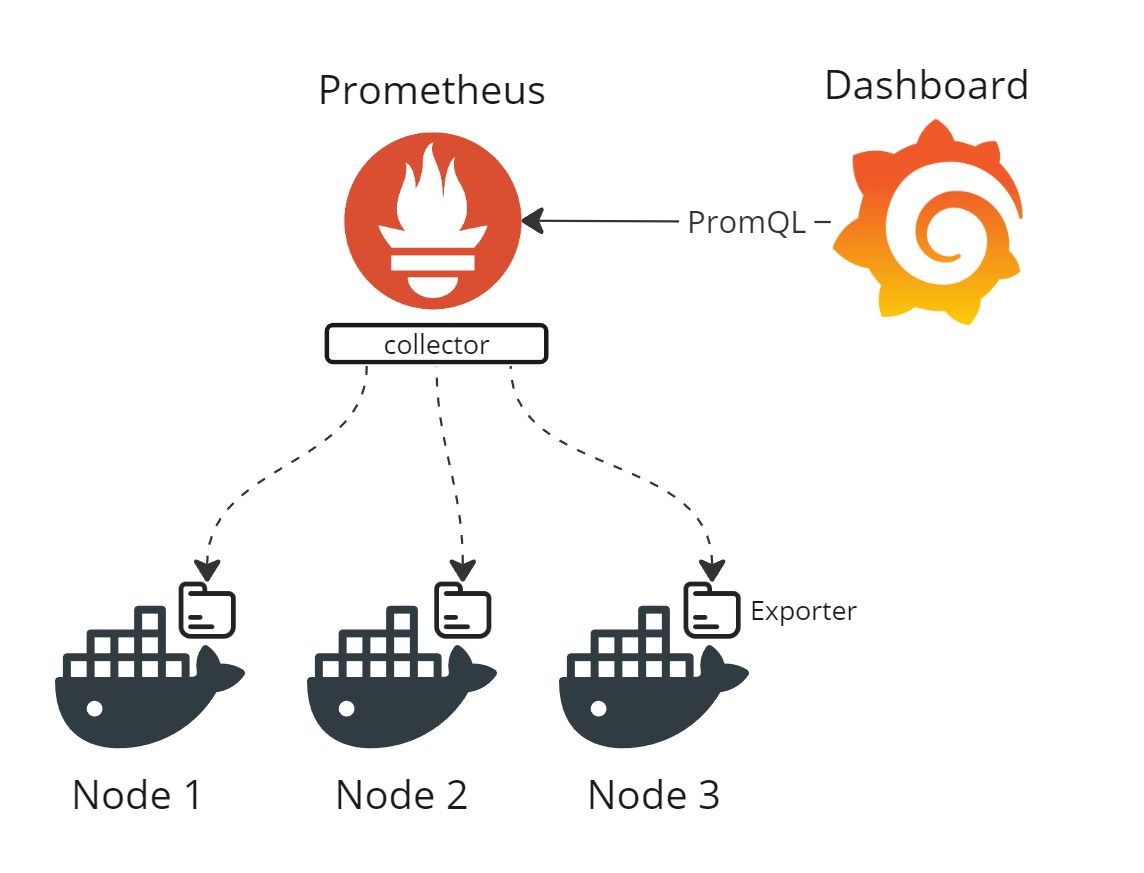
\includegraphics[width=0.75\linewidth]{Imagens/cap6/cap6instrumentalizacao.jpg} 
	
	Fonte: elaborado pelo autor.
\end{figure}


Com a necessidade de visualização dos dados durante execução, foi criado um quadro ( \textit{dashboard}) para apresentar os resultados obtidos de forma gráfica. Logo, com o auxilio do Grafana\footnote{disponível em: \url{https://grafana.com/}}, uma plataforma aberta para análise e visualização de dados em quadros personalizáveis. Foi concebida essa interface de acompanhamento do experimento e a Figura \ref{fig:cap6bashboard} apresenta em aspecto a configuração dos quadros criados. Para avaliação posterior após a execução do experimento, os dados foram exportados, e dispostos em planilha eletrônica capaz de produzir os gráficos necessários para análise dos resultados. 

\begin{figure}[H]
	\centering
	
	\caption{Dashboard para visualização dos resultados.}
	\label{fig:cap6bashboard}
	\noindent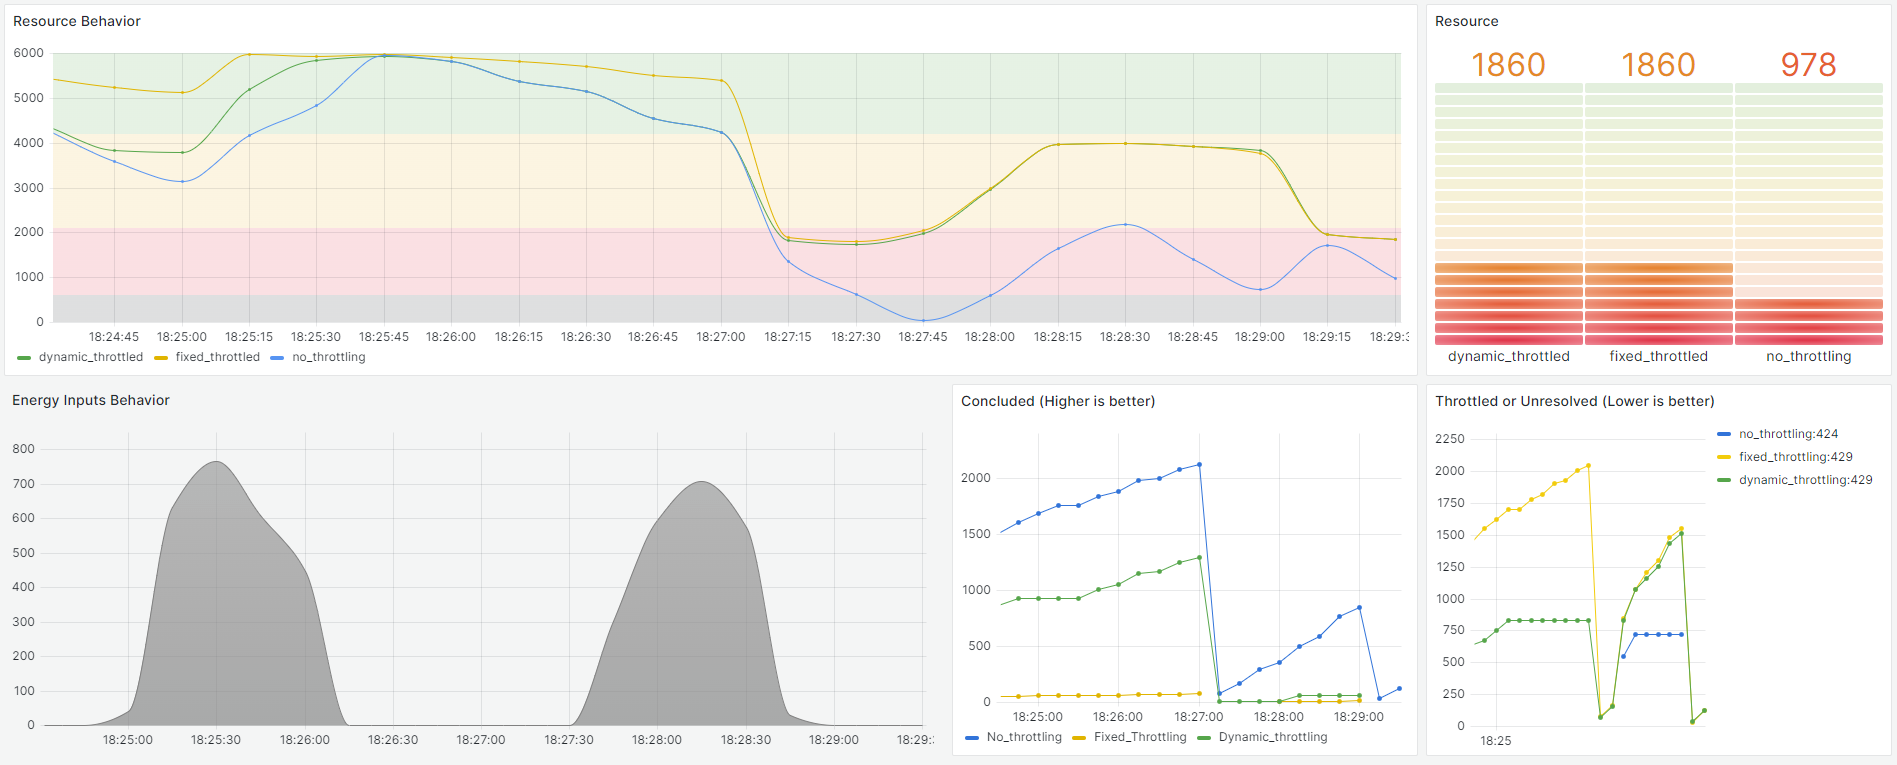
\includegraphics[width=1\linewidth]{Imagens/cap6/cap6dashboard.png} 
	
	Fonte: elaborado pelo autor.
\end{figure}

É pertinente ressaltar que os processos realizados para instrumentalização, em especial o \textit{exporter}, não exerce influência sobre a gasto energético simulado do dispositivo durante execução do experimento. Sua presença é transparente para a implementação, funcionando como um agente independente que não impacta nas dinâmicas energéticas colocadas em análise.

\section{Execução}
\label{cap6:execucao}

O estudo experimental foi realizado em etapas conforme descritos em referencia a Figura \ref{fig:cap6metodologia}, assim, as variáveis independentes descritas foram controladas para minimizar possível viés garantindo a consistência e replicabilidade do experimento. Durante a execução, os processos de instrumentalização atuaram em conformidade para que enquanto todos os dados necessários eram coletados, nenhuma variável externa pudesse influenciar nos resultados. Desta forma, as execuções contribuem para obtenção dos dados necessários para analisar e validar os resultados.

No inicio de uma execução, o \textit{storage} recebe o valor equivalente a sua capacidade máxima de armazenamento, a partir disso, os valores de oferta são disponibilizadas pelo \textit{power supply} e seguem a referencia apresentada na Tabela \ref{table:cap6distribuicaonatal}, assim, submetidos a medida que se inicia um novo ciclo $c_0, c_1,...,c_{23}$ relativos as jornada $J_1, J_2, ..., J_{12}$. Dado controle do experimento, a execução atende as características gerais de oferta de recursos com certa previsibilidade. Foram realizadas 3 execuções e seus resultados obtidos são em referencia dos mesmos valores fornecidos conforme descrito na Figura \ref{fig:cap6valoresofertados} na forma de variável independente.


Portanto, ao iniciar um ciclo $c$, o valor referente é entregue e, por sua vez, armazenado. Passados 6 segundos, um novo ciclo inicia-se encerrando o anterior em decorrência do novo valor ofertado. Este processo de iteração é referente aos ciclos de todas as jornadas e durará $\approx 1728 segundos$, tempo necessário para que o experimento apresente a atuação completa da dinâmica de estados e modos de operação possíveis.

\begingroup
\begin{table}[htbp]
	
	\centering
	\caption{Instanciação taxonômica dos dispositivos.}
	\small
	%	\tabcolsep=0.05cm
	\begin{tabular}{ c c c c c c c}
		\toprule
		Dispositivo & Nome & \textit{Throttling} & \multicolumn{4}{c}{Atuação}\\\cline{4-7}		
		& & & Limiar & Ciclos & Meios & Observáveis\\
		\midrule
		%		\hline
		disp$_1$ & no-throttling  & Não & - & 288 & - & - \\
		disp$_2$ & fixed-throttling  & Sim & Fixo & 288 & Vazão & - \\
		disp$_3$ & dynamic-throttling  & Sim & Adaptativo & 288 & Vazão & Reserva \\
		\bottomrule
	\end{tabular}
	\label{table:cap6:dispositivosutilizados}
	\\
	\footnotesize Fonte: elaborado pelo autor.
	
\end{table}
\endgroup

O dispositivo disp$_1$, representa o comportamento de dispositivos sem nenhum mecanismo de limitação das solicitações, seu objetivo principal é servir como base de comparação a medida que deverá atender todas as demandas solicitadas sem restrições previamente estabelecidas, com a observação de que caso seu valor armazenado em \textit{storage} seja completamente consumido, caracterizará esgotamento energético, incapacitando o dispositivo a atender qualquer tipo de solicitação.

Por sua vez, disp$_2$  e disp$_3$ foram implementados com a capacidade de limitar suas operações. Entretanto a atuação do mecanismo \textit{throttling} é distinta entre eles, para o disp$_2$ é realizada restrição mediante limiar fixado apenas em razão da uma vazão de atendimento estipulada previamente sem observar adequação ao cenário energético ou privilégios do solicitante. Por sua vez, cabe a atuação do limiar no disp$_3$ atuar adaptativamente assim como no anterior regulando a taxa de vazão de atendimento porém observando as condições de sua reserva em \textit{storage}.Sendo assim, a relação entre os modos de operação e o comportamento do limitador, quando presente, esta referenciado na Tabela \ref{table:cap6:expectativasolicitacoes}.

\begingroup
\begin{table}[h] \centering
	\caption{Expectativa de atendimento das solicitações ($sol$) por ciclo ($c$)}
	\small
%	\tabcolsep=0.05cm
	\begin{threeparttable}
	\begin{tabular}{ l c c c c c}
		\toprule
			Nome &
			\textit{Throttling   } & 
			\multicolumn{4}{c}{Modo de Operação}\\\cline{3-6}
			& &  \begin{tabular}{@{}c@{}} Abundante \\ {\tiny(\textit{S\tnote{*}} $\ge$ 70\% )} \end{tabular} &
			\begin{tabular}{@{}c@{}} Atenção \\ {\tiny(70\% > \textit{S} $\ge$ 50\%)} \end{tabular} &
			\begin{tabular}{@{}c@{}} Alerta \\ {\tiny(50\% > \textit{S} $\ge$ 10\%)} \end{tabular} &
			\begin{tabular}{@{}c@{}} Hibernando \\ {\tiny( 10\% > \textit{S} $\ge$ 0\%)} \end{tabular} \\
		\midrule
		 no-throttling &Não & 30 $sol/c$ & 30 $sol/c$ & 30 $sol/c$ & 30 $sol/c$ \tnote{**} \\
		 fixed-throttling & Sim & 15 $sol/c$ & 15 $sol/c$ & 15 $sol/c$ & 0 $sol/c$\\
		 dynamic-throttling & Sim & 30 $sol/c$ & 22 $sol/c$ & 15 $sol/c$ & 0 $sol/c$\\
		
		\bottomrule 
	\end{tabular}
	\begin{tablenotes}\footnotesize
		\item[*] \textit{S} representa o percentual do total energético armazenado em  \textit{storage} no momento observado.
		\item[**] Ao atingir 0\% o dispositivo estará esgotado e atenderá 0 $sol/c$.
	\end{tablenotes}
\end{threeparttable}
	\label{table:cap6:expectativasolicitacoes}
	\\
	\footnotesize Fonte: elaborado pelo autor.
\end{table}
\endgroup

\begin{comment}
Em resumo, cada execução do experimento carrega as características conforme os itens abaixo:

\begin{itemize}
	
	\item \textbf{Total de ciclos:} 288 ciclos
	\[
	\text{TotalCiclos} = 12 \, \text{jornadas} \times 24 \, ciclos/jornada = 288 ciclos
	\]
	\item \textbf{Razão das Solicitações:} $\approx$5 \,\text{solicitações/s} 
	\[
	\text{RazãoSolicitações} = \frac{30 \, \text{solicitações}}{6 \, \text{s}} \approx 5 \, \text{solicitações/s}
	\]
	\item \textbf{Total de solicitações:} $\approx$8640 solicitações
	\[
	\text{TotalSolicitações} = 288 \, \text{ciclos} \times 30 \, \frac{\text{solicitações}}{\text{ciclo}} \approx 8640 \, \text{solicitações}
	\]
	
	\item \textbf{Tempo de Execução:} $1728 \ segundos$
	\[
	 Tempo Execução = 12 \, \text{jornadas} \times \text{Total de Ciclos} \times 6 = 1728 \ segundos \ (28min \ 48seg)
	\]
	

\end{itemize}
\end{comment}

Finalmente, o gasto dos recursos é obtido a partir da dinâmica de estados ativo-inativo-hibernando e as condições para permanecer em um determinado estado conforme Figura \ref{fig:cap6maquinaestados}, sendo assim, ao logo de um ciclo, o dispositivo que permanecer ativo durante todo tempo despenderá sua reserva de maneira  acentuada quando comparado a outro dispositivo que optou permanecer parcialmente inativo. Toda requisição realizada enquanto um dispositivo esteja em estado Hibernando,  sem reserva suficiente para manter-se operacional, será considerada não atendida em razão da indisponibilidade do dispositivo por esgotamento.

\section{Avaliação dos Resultados}
\label{cap6:avaliacao}

Durante a atividade de avaliação dos resultados, examina-se em detalhes os valores obtidos a partir das execuções do experimento. Descreve-se os dados coletados que compõe as variáveis independentes em função dos valores utilizados e também é apresentado os valores das variáveis dependentes coletadas com o objetivo de validar o experimento. 
Parte da avaliação se concentra em apresentar descritivamente os dados coletados, a interpretação dos resultados e por fim, as limitações do estudo experimental.



\subsection{Descrição dos Dados Coletados}

A Figura \ref{fig:cap6valoresofertados}, apresenta o aspecto da distribuição dos valores ofertados aos dispositivos durante o experimento. Estes, quantificaram a primeira variável independente e são utilizados para definir como foi realizada a disponibilização de recursos através do \textit{power supply} no decorrer do tempo, sendo estes disponibilizados estritamente no inicio de cada ciclo. Sendo o primeiro valor no ciclo $c_{0}$ da jornada $J_1$ e, por sua vez, o ultimo transmitido no inicio do ciclo $c_{23}$ da jornada $J_{12}$. Decorrido o tempo disposto para o ultimo ciclo da jornada $J_{12}$, finda-se a execução do experimento.

\begin{figure}[H]
	\centering
	
	\caption{Entradas fornecidas ao storage dos dispositivos.} 
	\label{fig:cap6valoresofertados}
	\noindent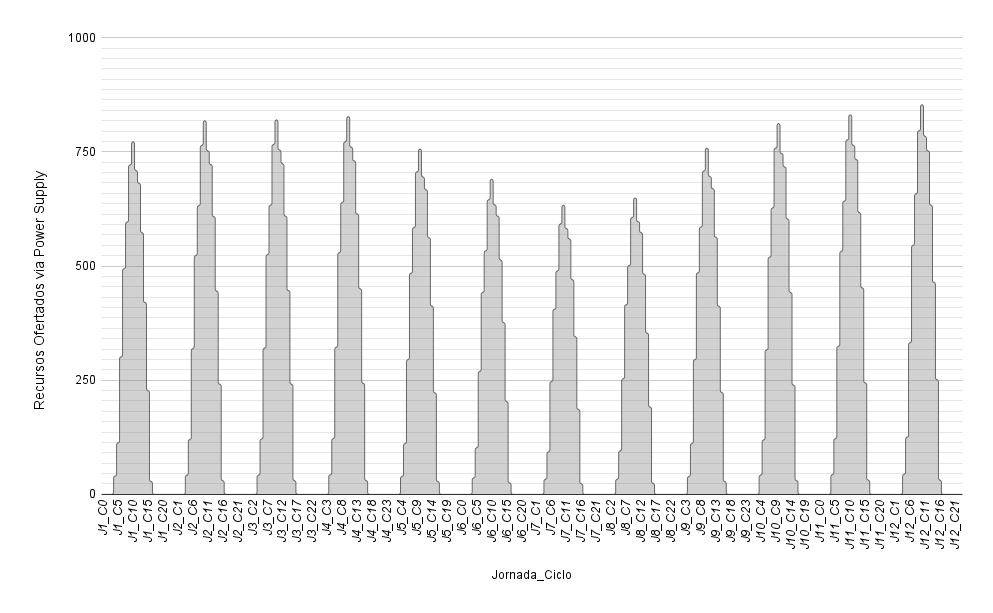
\includegraphics[width=1\linewidth]{Imagens/cap6/cap6valoresofertados.png} 
	
	Fonte: elaborado pelo autor.
\end{figure}

Dada a natureza do experimento, toda execução obtêm o mesmo comportamento da oferta energética conforme distribuição definida. Assim os valores já seguem definidos antes da execução e não sofrem impacto diante das características dos dispositivos no contexto de uma ou outra execução. Além disso, é garantido ao dispositivo receber este valor mesmo que esteja momentaneamente esgotado, pois não configura uma solicitação.

A segunda variável independente utilizada, representa as solicitações disparadas contra a interface do dispositivo provedor. Este estimulo tem características tais que, ao atender-las, o provedor intensifica seu consumo energético, pois encontra-se em estado ativo, demandando mais recursos. Isso implica que, à medida que a quantidade das solicitações atendidas aumenta, o consumo de energia do provedor também aumentará proporcionalmente, resultando em um impacto significativo na disponibilidade do dispositivo em relação com seu desempenho energético. A Tabela \ref{table:cap6:execucaocaracteristicas}, apresenta os valores utilizados para as requisições em cada execução do experimento. A precisão indica a distribuição da relação entre total de solicitações em cada execução em referencia para 12 jornadas (8640 solicitações) descrito na Seção \ref{cap6:execucao}.

\begingroup

\begin{table}[h]
	
	\centering
	\caption{Solicitaçoes realizadas}
	\begin{threeparttable}
	\begin{tabular}{ l c c c c }
		\toprule
		&   & \multicolumn{3}{c}{Solicitações ($sol$)}\\\cline{3-5} & Duração&
		\begin{tabular}{@{}c@{}} Execução 1\end{tabular} & \begin{tabular}{@{}c@{}} Execução 2\end{tabular} & \begin{tabular}{@{}c@{}} Execução 3\end{tabular}\\
		\bottomrule
		1 ciclo  				& 6 $seg$ 	& 29,875 	& 29,86 & 29,88 \\
		1 Jornada (24 ciclos)  	& 144 $seg$	& 717 & 716,75 &  717,16\\
		12 Jornadas  			& 1728 $seg$& 8604  & 8601 & 8606 \\
		\bottomrule
	\end{tabular}

	\end{threeparttable}
	\label{table:cap6:execucaocaracteristicas}
	\\
	\footnotesize Fonte: elaborado pelo autor.
	
\end{table}
\endgroup


Ao finalizar uma execução, as variáveis dependentes obtidas são colhidas para avaliação: a quantidade total de solicitações atendidas ao fim da execução do experimento e a evolução desses valores; a quantidade de solicitações impedidas mediante indisponibilidade do dispositivo por esgotamento. Para analisar a diferença na quantidade de solicitações atendidas, é necessário contrapor dados de reserva em \textit{storage} com os valores ofertados pelo \textit{power supply}, assim buscará justificará na atuação de limitadores.	

Ainda sobre os dados coletados, ao final de cada execução é obtido o total de requisições atendidas evidenciando como as características dos agentes limitantes agem sobre a performance dos dispositivos. Na Figura \ref{fig:cap6solicitacoesatendidas}, é possível comparar o desempenho dos dispositivos sob a ponto de vista das solicitações atendidas.

\begin{figure}[H]
	\centering	
	\caption{Quantidade de solicitações atendidas por dispositivo.} 
	\label{fig:cap6solicitacoesatendidas}
	\noindent\includegraphics[width=0.8\linewidth]{Imagens/cap6/cap6solicitaçoesatendidas_execs.png} 
	
	Fonte: elaborado pelo autor.
\end{figure}



Apenas o dispositivo "no-throttling" apresentou em seu resultado um valor de indisponibilidade em função de esgotamento energético, de modo geral a Tabela \ref{table:cap6:quadrogeralobtido} apresenta a performance dos dispositivos em razão das solicitações atendidas e também resume os valores de solicitações que obtiveram cenário de indisponibilidade em razão do total de solicitações realizadas.

\begingroup
\begin{table}[H]
	\centering
	\caption{Quadro das solicitações realizadas aos dispositivos}
	\begin{tabular}{|c|c|c|c|c|c|}
		\hline
		\multirow{2}{*}{Execução} & 
		\multirow{2}{*}{Dispositivo} &
		\multicolumn{4}{c|}{Solicitações}  \\\cline{3-6}\addlinespace[1pt]
		& & realizadas&  atendidas & indisponíveis  & \% indisponíveis \\
		\hline\addlinespace[1pt]
		\multirow{3}{*}{1} 	& no-throttling 	& 8604 &  7043	& 1561 	 	& 0.1814\\
							& fixed-throttling 	& 8604 &  3414	& 0 		& -\\
							& dynamic-throttling & 8604 & 5098 & 0 		&-\\
		\hdashline\addlinespace[1pt]
		\multirow{3}{*}{2}	& no-throttling 	& 8601 & 7105	& 1496  & 0.1739\\
							& fixed-throttling 	& 8601& 3436	& 0  & -\\
							& dynamic-throttling & 8601 & 5118	& 0  &-\\
		\hdashline\addlinespace[1pt]
	   \multirow{3}{*}{3}  & no-throttling & 8606 & 7105& 1504 &0.1747\\
	   	& fixed-throttling & 8606 &3441 & 0& -\\
	   	& dynamic-throttling & 8606 & 5123& 0&-\\
		\hline

	\end{tabular}
		\label{table:cap6:quadrogeralobtido}
		\\
		\footnotesize Fonte: elaborado pelo autor.
\end{table}
\endgroup

Parte da análise é obtida ao observar o gráfico de comportamento referente às capacidades energéticas encontradas no \textit{storage} do dispositivo. A Figura \ref{fig:cap6recortecomportamentostorage} apresenta um recorte dos dados, oferecendo informações suficientes para inferências sobre a dinâmica entre a coleta e a forma de consumo de recursos por todos os dispositivos envolvidos. Essa visualização permite identificar alguns padrões de consumo e tendências de eficiência especialmente nas áreas em destaques verticais que destacam a quantidade minima de recurso disponibilizado.

\begin{figure}[H]
	\centering	
	\caption{Recorte do comportamento da oferta e uso dos recursos durante execução.} 
	\label{fig:cap6recortecomportamentostorage}
	\noindent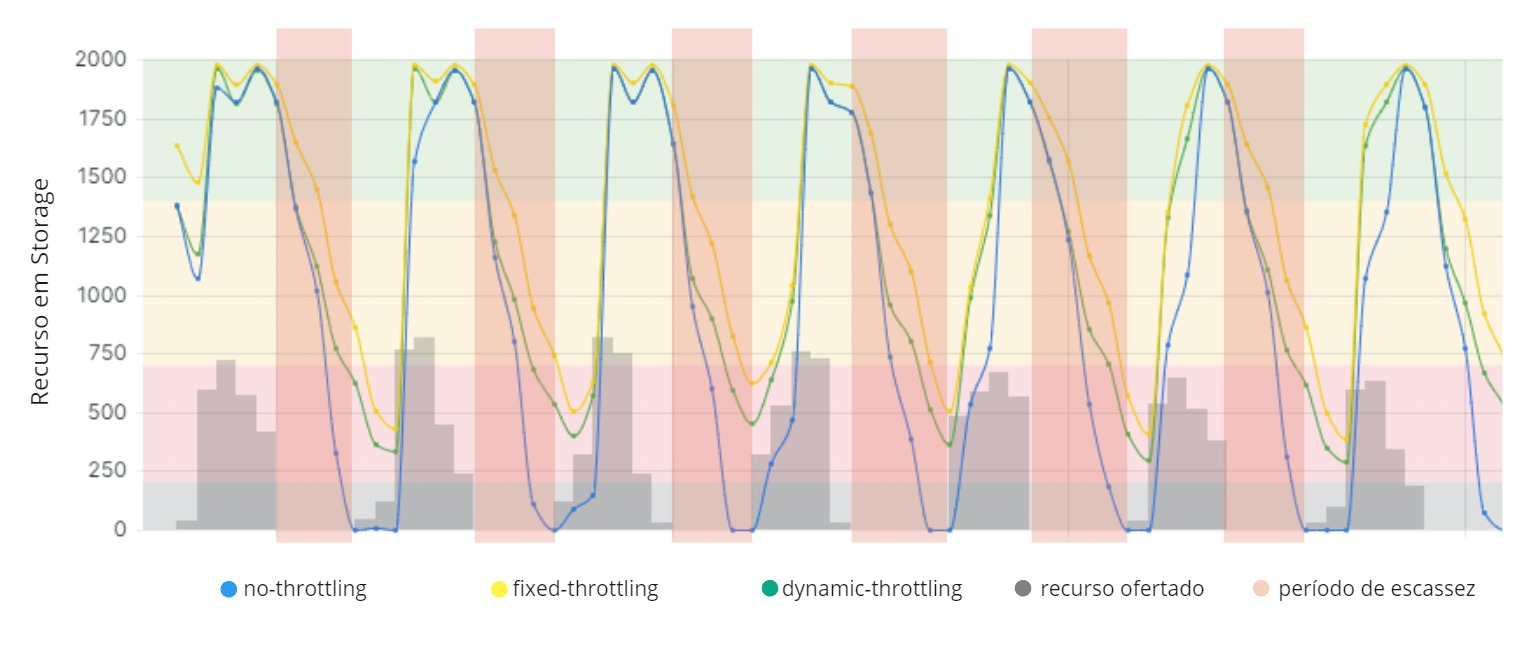
\includegraphics[width=1\linewidth]{Imagens/cap6/cap6recortecomportamentostorage.jpg} 
	
	Fonte: elaborado pelo autor.
\end{figure}

A análise realizada sobre a Figura \ref{fig:cap6recortecomportamentostorage} permite a visualização clara do comportamento do dispositivo \textit{dynamic-throttling} enquanto a atuação é adaptada em cada modo de operação com referencia a sua condição apresentada em \textit{storage}, este processo é notável através do amortização na tendencia da linha de consumo enquanto alterna-se as faixas horizontais definidas na relação de cores e representam os modos de operação implementados para experimentação. Sendo assim:

\begin{itemize}
	\item Zona Verde, representa faixa de atuação em modo Abundante;
	\item Zona Amarelo, representa faixa de atuação em modo Atenção;
	\item Zona Vermelho, representa faixa de atuação em modo Alerta;
	\item Zona Cinza, representa faixa de Hibernação e seu esgotamento energético.
\end{itemize} 

\subsection{Interpretação dos Resultados}
\begin{comment}
	Descreva os resultados dos testes de uma maneira que seja compreensível para o leitor. Discuta se os resultados foram estatisticamente significativos e o que isso significa em termos do seu experimento.
\end{comment}

Com as execuções realizadas, é possível inferir sobre como os dispositivos são afetados pelas características dos fatores energéticos aos quais estão expostos. Através dessas execuções, podemos analisar de que forma a energia ofertada durante o experimento impactou no desempenho dos dispositivos permitindo uma compreensão aprofundado profunda dos seus comportamentos e limitações principalmente em ambientes em condições menos preditivas ou controladas.

Ao categorizar um dispositivo \acs{IoT} com capacidade de coleta, é preciso fazer menção sobre o papel que este irá desempenhar. Para isso, o experimento atuou gerando cenário para que os agentes examinados pudessem cumprir o papel de provedor desde o momento que este dispositivo é configurado para atender solicitações.

Os resultados obtidos, descrevem a importância dos elementos categorizados em função das características encontradas nos trabalhos relacionados à dispositivos para computação dirigida à energia, a medida que observam-se o comportamento fatores energéticos e os impactos relacionados a busca por evitar um esgotamento energético.

Sobre a capacidade de atender solicitações, a análise do uso de recursos utilizados pelo dispositivo 'no-throttling' na Figura \ref{fig:cap6nothrottling} destaca que a continuidade no seu desempenho para atender solicitações é fortemente impactada pelos valores energéticos coletados. Por não possuir nenhum agente limitador experimentado, o dispositivo tem a capacidade de utilizar seus recursos de forma irrestrita, mesmo em cenários de escassez. No entanto, isso pode conduzi-lo à estado de esgotamento, onde ele perde a capacidade de realizar qualquer ação, mesmo um eventual contingenciamento dos efeitos da indisponibilidade, o que pode ter consequências graves.

\begingroup
\begin{figure}[htb]
	
	\centering
	\caption{Aqui vou colocar uma figura para isolar o comportamento do no-throttling.}
	\label{fig:cap6nothrottling}
	\noindent\includegraphics[width=0.3\linewidth]{example-image} 
	
	Fonte: elaborado pelo autor.
\end{figure}
\endgroup



Posteriormente, ao instanciar os dois dispositivos com diferentes limitadores, com o pretexto de validar a aderência dos conceitos classificados na taxonomia proposta. Os dados obtidos oriundos da experimentação colaboram com o entendimento dos elementos envolvidos no processo de concepção de um dispositivo sobretudo dada necessidade de implementar os mecanismos de limitação para lidar com os aspectos de disponibilidade.

Em relação ao comportamento esperado dos dispositivos, nota-se que o mecanismo \textit{throttling} exerceu influência ativa como candidato para adequação de comportamento, sobretudo quando considera-se os aspectos dos recursos energéticos envolvidos, necessários para alcançar um grau de disponibilidade estimado em requisito de qualidade do serviço (\acl{QoS}). Ainda sobre estes termos, confrontam-se o desempenho obtido pelos dispositivos 'fixed-throttling' e 'dynamic-throttling', na Figura \ref{fig:cap6fixedxdynamic} percebe-se a necessidade de alinhamento sobre a forma como o limitador deverá agir em respeito aos meios possíveis em concordância com resultados esperados.

Graças a isso, é possível perceber que o dispositivo 'fixed-throttling' obteve menor variação de sua reserva energética, porque se valendo da periodicidade da condição de oferta, teve o \textit{throttling} atuando fixamente durante os ciclos, e assim, de maneira constante consumiu seus recursos ao passo que também atendia as solicitações em termos dos limites da taxa de vazão sobre os meios desse dispositivo provedor sem observar necessariamente nenhum critério observável categorizado. 
 
\begingroup
\begin{figure}[htb]
	
	\centering
	\caption{Comparação comportamento das estratégias de throttling aplicadas.}
	\label{fig:cap6fixedxdynamic}
	\noindent\includegraphics[width=0.3\linewidth]{example-image} 
	
	Fonte: elaborado pelo autor.
\end{figure}
\endgroup

Ainda em relação à Figura \ref{fig:cap6fixedxdynamic} é correto afirmar também que a diferença de comportamento do dispositivo 'dynamic-throttling' em relação à outra implementação com limites fixos, foi proporcionada pela capacidade incrementada ao \textit{throttling} em observar os fatores de sua reserva energética. Com isso incrementou sua habilidade de gerenciamento sobre os recursos apoiando por simples \acs{QoS} presente e atuante na forma de modo de operação, característica viabilizante da capacidade adaptativa. De modo que, apesar dos momentos de escassez, o dispositivo foi capaz de manter-se disponível energeticamente e ainda obter o total de solicitações atendidas superiores aos obtidos pela abordagem do dispositivo que utiliza limitador fixo em função unicamente da vazão de atendimento.
 

Em todo caso, é prematuro afirmar com base apenas na experimentação, que um dispositivo é simplesmente mais disponível que outro, e de fato não é objetivo do experimento encontrar a melhor implementação. Pois, o numero superior de solicitações atendidas atribuídas ao dispositivo 'no-throttling' não reflete outros critérios de disponibilidade não experimentados e possivelmente descritos na forma de \acs{SLA}.

Entretando, o simples fato de apresentar intermitência de operação, recorrentemente presente periodicamente quando submetido em cenário de escassez da fonte energética gera indícios que podem ser consideravelmente indesejados ou não tolerados. Caberá o apoio do agente definidor dos termos de operação esperados para fundamentalmente descrever a criticidade e a tolerância para os momentos de indisponibilidade energética bem como da operação como todo. 

Finalmente, as instancias experimentadas apresentam, evidenciado pelos resultados obtidos, as referências aos atributos listados para o uso de throttling como atuador em busca de atender critérios de disponibilidade, especialmente para computação dirigida à energia necessária para dispositivos \acs{IoT}. Por isso,  clarifica a ideia de atenção sobre os elementos ligados taxonomicamente ao \textit{throttling} quanto a aplicação mediante analise cuidadosa dos termos de serviço necessários para definir uma configuração de atuação para alcançar disponibilidade esperada.



\subsection{Limitações do Estudo}
\begin{comment}
	Reconheça quaisquer limitações do seu estudo que possam ter afetado os resultados. Isso pode incluir limitações metodológicas, questões de amostragem, viéses potenciais ou qualquer outra consideração importante.
\end{comment}

As limitações do experimento, passam especialmente pela não examinação de cenários derivados dos estados fundamentais atribuídos para um dispositivo conforme descrito. Apesar de expressar bem a intenção proposta, um dispositivo pode ter níveis de atividades diferentes os quais poderiam ser melhor evidenciados pelo uso de mais de uma interface de acesso ao dispositivo, de tal forma que a configuração de custo teria mais possibilidades mediante nivel de atividade empregado no dispositivo.

Algumas características da taxonomia não foram cobertas totalmente no experimento, não é possível examinar o ponto de vista do consumo energético dos agentes enquanto clientes. A definição de protocolo de comunicação também acabou por inviabilizar alguns cenários.





 